\section{Multi dimensional inputs and outputs}
\begin{frame}{Using vectors}

		\begin{block}{$x \in \mathbb{R}^n$,$y \in \mathbb{R}^m$, $w\in \mathbb{R}^{m \times n}$}
			\begin{align*}
				\begin{bmatrix}
					y_1 \\
					y_2 \\
					\vdots \\
					y_m
				\end{bmatrix} & =  
				\begin{bmatrix}
					w_{11} & w_{12}& \dots & w_{1n}  \\
					w_{21} & w_{22}& \dots & w_{2n}  \\
					\vdots &\vdots &  & \vdots  \\
					w_{m1} & w_{m2}& \dots & w_{mn}  \\
				\end{bmatrix}
			\begin{bmatrix}
				x_1 \\
				x_2 \\
				\vdots \\
				x_n
			\end{bmatrix} + 
			\begin{bmatrix}
			b_1 \\
			b_2 \\
			\vdots \\
			b_n
			\end{bmatrix}
			\end{align*}
		For $m=2, n=3$
		\begin{align*}
		y_1 &= w_{11}x_1 + w_{12}x_2+w_{13}x_3 + b_1 \\
		y_1 &= w_{21}x_1 + w_{22}x_2+w_{23}x_3 + b_2 
		\end{align*}
		\end{block}
\end{frame}
\begin{frame}{Mandatory network diagram}
	
\includegraphics[width=.6\textwidth, center]{figuras/fully_connected_0_layer.png}	
\end{frame}
\begin{frame}{More layers}
	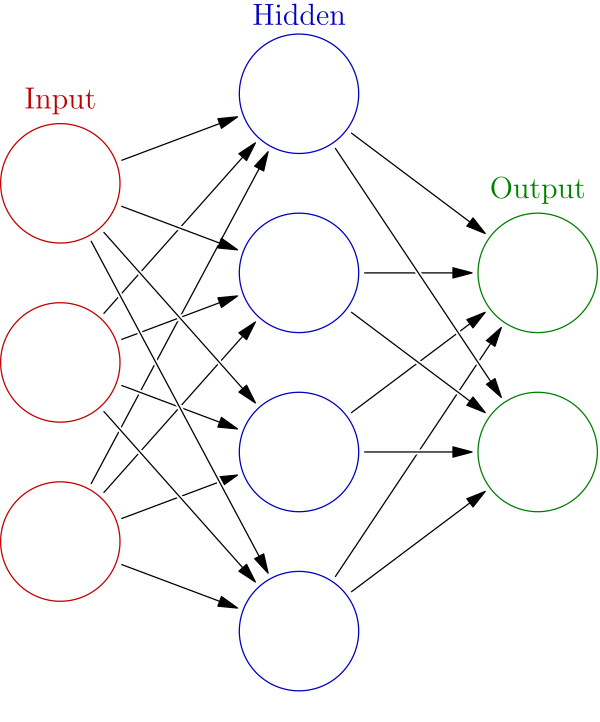
\includegraphics[width=.5\textwidth, center]{figuras/Colored_neural_network_1_hidden.png}
	\tiny{https://en.wikipedia.org/wiki/Artificial\_neural\_network }
\end{frame}
\begin{frame}{Multiple layers}
	\begin{block}{Layers (composition) of $ax+b$ style functions}
		\begin{align*}
		y &= \mathbb{W} x + b  \\
		z &= \mathbb{U} y + c =\mathbb{U}(\mathbb{W}x+b)+c \\
		  &= (\mathbb{U}\mathbb{W})x + (\mathbb{U}b+c) = \mathbb{V}x+d 
		\end{align*}
	\end{block}
	\begin{block}{Introducing non-linearity with element-wise sigmoid}
		\begin{align*}
		y &= \mathbb{W}x+b \\ 
		z &= \sigma(y) 
		\end{align*}
	\end{block}
\end{frame}
\begin{frame}{Multi-layer, feed forward, non-polynomial}
	%\begin{block}{Multi-layer, feed forward network with non-polynomial activation}
		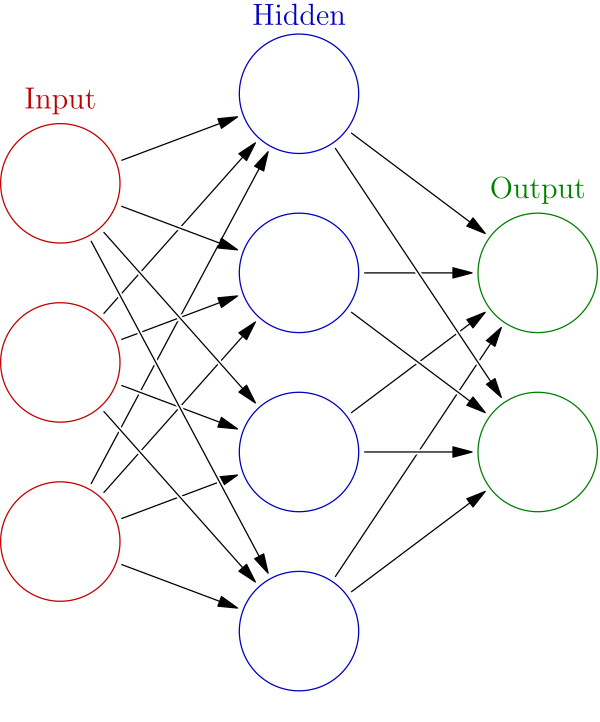
\includegraphics[width=.4\textwidth, center]{figuras/Colored_neural_network_1_hidden.png}
		\tiny{Image from: https://en.wikipedia.org/wiki/Artificial\_neural\_network }
	%\end{block}
	
\end{frame}

\begin{frame}{What can this neural network do?}
\begin{quote}
	{\small
		A standard multilayer feedforward network with a locally bounded 
		piecewise continuous activation function can approximate any continuous 
		function to any degreeof accuracy if and only if the network's activation 
		function is not a polynomial.\\
		-Leshno et al.,1993
	}
\end{quote}
\begin{quote}
	{\small 
	In particular, we show that arbitrary decision regions can
	be arbitrarily well approximated by continuous feed forward neural networks with
	only a single internal, hidden layer and any continuous sigmoidal nonlinearity.\\
	-Cybenko, 1989 
	}
\end{quote}
\end{frame}